\chapter{Introdución}
\label{chap:introducion}

\lettrine{P}{rimer} capítulo da memoria


\section{Contexto xeral}
\label{sec:mostra}

\nota{Este párrafo igual non me quedou ben pero ghustaríame empezar con algo así máis ou menos de contexto histórico, porque paréceme importante. Non gustaríame soar prepotente por outra banda...}

No contexto das sociedades da información que levamos vivindo como mínimo dende a revolución industrial, é cada vez máis evidente a importancia do \acrfull{apraut}. Esta disciplina que trata de \textit{aprender} funcións (de calquera propósito) en base a unha experiencia o un conxunto de datos (de calquera orixe), gozou dun esplendor tanto no desenvolvemento teórico como nas aplicacións durante a segunda metade do pasado século~\cite{vapnik95}. Hoxe, na tercera década do século XXI atopamos que a natureza dos datos trocou, onde denantes unha representación natural dos datos era útil e con garantías de éxito, agora con datos multimodais, que xurden da interacción social é máis difícil. En particular os dominios das nosas funcións poden ser espazos moi complexos e os datos de entrada poden precisar un preprocesado particular. Se antes a disciplina de \acrfull{dsp} ofrecía unha serie de métodos de preprocesado (Filtrado de Kalman, Transformada de Ondas Discreta...), agora o \acrfull{ar} ofrece unha serie de métodos para \emph{aprender} o preprocesado axeitado para a combinación de tarefa e conxunto de datos. É por isto que recentemente estase a ver un crecemento moi acelerado no \acrfull{aprpro}, unha subdisciplina do \acrshort{apraut} que ten como \textit{slogan}: ``Máis grande é mellor''~\cite{alexnet, vgg} e prentende solventar o problema do \acrshort{ar} a través dunha sucesión de operadores non lineais coñecidos como \acrfull{rna}.

Pola súa banda as compoñentes das \acrshort{rna} actuais non gozan da mesma xustificación teórica que acostumaban antaño outros algoritmos de \acrshort{apraut}, como a Regresión Lineal ou as Máquinas de Soporte Vectorial~\cite{vapnik95}. Por tanto vivimos nun momento no que as \acrshort{rna} reinan o mundo das aplicacións pero sen que  exista unha teoría conclusiva que as avale, ou cando menos de momento. Esta situación motivou o desenvolvemento dun marco para comprender as \acrshort{rna}, primeiro dende o punto de vista do algoritmo, é dicir \gls{interpretabilidade} dos seus procesos de aprendizaxe e inferencia, para finalmente poder entender as decisións que toma de xeito individual e ofrecer unha xustificación a devandita resposta, é dicir, \gls{explicabilidade}~\cite{Wright_2022}.

\section{Revisión pormenorizada SOTA e traballos relacionados}
O traballo neste TFG móntase sobre a arquitectura CRATE (ver \ref{subsec:crate}, páxina \pageref{subsec:crate}). Para poder exponer tanto a devandita arquitectura como as nosas aportacións, é necesaria a revisión duns conceptos previos.
\subsection{ISTA}

Un algoritmo clásico do \acrshort{apraut} é a Regresión Lineal, co que Carl F. Gauss empezou a teorizar e ofrecer garantías sobre o seu modelo \[X\beta = Y + \epsilon\] onde $\epsilon \sim \mathcal{N}(\mu, \sigma^2)$ nos albores do século XIX, chegando á coñecida forma cerrada \[\hat\beta = (X^{'}X)^{-1}X^{'}Y.\] A primeira regularización do modelo para facelo máis robusto chegou con ideas orixais no campo de resolución de problemas mal planteados, Andrey Tikhonov introduce a penalización segundo a norma $\mathcal{L}_2$ dos parámetros $\beta$, o cal é equivalente a asumir unha distribución Gausiana en $\beta$. O estimador ten a forma cerrada \[\hat\beta = (X^{'}X +\lambda I)^{-1}X^{'}Y\]  onde $\lambda$ controla a estructura do conxunto de funcións~\cite{vapnik95}. Se ben esta regularización segue a usarse hoxe en día porque devandita asunción pode ser moi natural, dende o 1996 considérase o \textsc{Lasso}~\cite{lasso}, que penaliza a norma $\mathcal{L}_1$ (equivalente a asumir unha distribución Laplaciana nos parámetros) e sen ter forma cerrada ofrece un estimador con ceros, é dicir o proceso de optimización de \textsc{Lasso} supón unha selección de características.

Como en moitas situacións de interese científico e comercial a resolución deste problema convexo por medio de métodos de punto interior pode ser infactible~\cite{beck2009fast}, o algoritmo \textsc{Ista} atopa unha solución ó \textsc{Lasso} a través da iteración: \[\beta_{t+1} = \sigma_{\epsilon}(\beta{t} - \lambda X^{'}(X\beta - Y)) \] onde $\sigma_{\epsilon}$ é a función de umbral suave (ver figura \ref{fig:funcions_activacion})


\begin{figure}[h]
  \centering
  
\includegraphics[width=0.75\textwidth]{imaxes/funcions_activacion.drawio.pdf}
	\caption{Funcións de activación usadas no traballo. (\textit{esquerda}) Función identidade (\textit{centro}) Función de umbral suave $\sigma_\epsilon(\cdot)$, parametrizada por $\epsilon$ (\textit{dereita}) Función ReLU, nótese que a función $\sigma_\epsilon(x)$ é indentica (no dominio $\mathbb{R}^{+}$) a  ReLU($x - \epsilon$).}
  \label{fig:funcions_activacion}
\end{figure}

\subsection{\textsc{MCR}$^{2}$ e ReduNet - Redes Caixa Blanca }

Na primeira metade da pasada década viuse o esplendor dun tipo de \acrshort{rna} nas que o operador principal é a convolución dun filtro ou \emph{kernel} aprendible coa imaxe (ou ca saída doutra convolución), estas Redes chámanse \acrfull{cnn}. Se ben son algo explicables \cite{visualizar_cnn, gradcam}, a pregunta `Que esta a facer esta compoñente da \acrshort{cnn}?' en xeral só pode responderse \emph{a posteriori}. Isto motivou ó grupo do profesor Yi Ma o desenvolvemento dunha \acrshort{cnn} como instancia do \acrshort{mcr2}~\cite{redunet}, creando así unha Rede Caixa Blanca \nota{acronimo? mellor en inglés?}.

A \acrfull{mcr2} é unha función obxectivo de \acrshort{ar} que intenta cumplir cos seguintes obxectivos na representación no espacio de características:

\nota{estas tres características sacoas de \href{https://arxiv.org/pdf/2311.13110}{o artigo de CRATE} pero quito a de `consistent' porque penso que non ven ó caso, \href{https://book-wright-ma.github.io/Book-WM-20210422.pdf}{no libro de 2022} fala doutras tres características, pero estas parécenme máis entendibles}

\begin{itemize}
				\item \emph{\textcolor{udcpink}{Comprimidas:}} sendo uniformemente distribuídas segundo algunhas estruturas de baixa dimensión\footnote{Como unhas gausianas} estándar que se axustan á baixa dimensionalidade intrínseca dos datos, co fin de asegurar unha codificación compacta dos datos.
				\item \emph{\textcolor{ficblue}{Lineais:}} as estruturas de baixa dimensión teñen unha xeometría (a anacos) lineal, co fin de facilitar a interpolación e a extrapolación no espazo de representación.
				\item \emph{\textcolor{udcgray}{Dispersas:}} as estruturas de baixa dimensión correspondentes a diferentes partes da distribución dos datos son estatísticamente incoherentes ou xeometricamente ortogonais, e tamén aliñadas cos eixes, co fin de asegurar unha codificación máis compacta e facilitar o procesamento posterior.
\end{itemize}

Formalmente defínese como a maximización da seguinte función: \[\Delta R (Z | \Pi_{[K]}) = R(Z) - R^{c}(Z | \Pi_{[K]})\]

\begin{figure}[h]
  \centering
  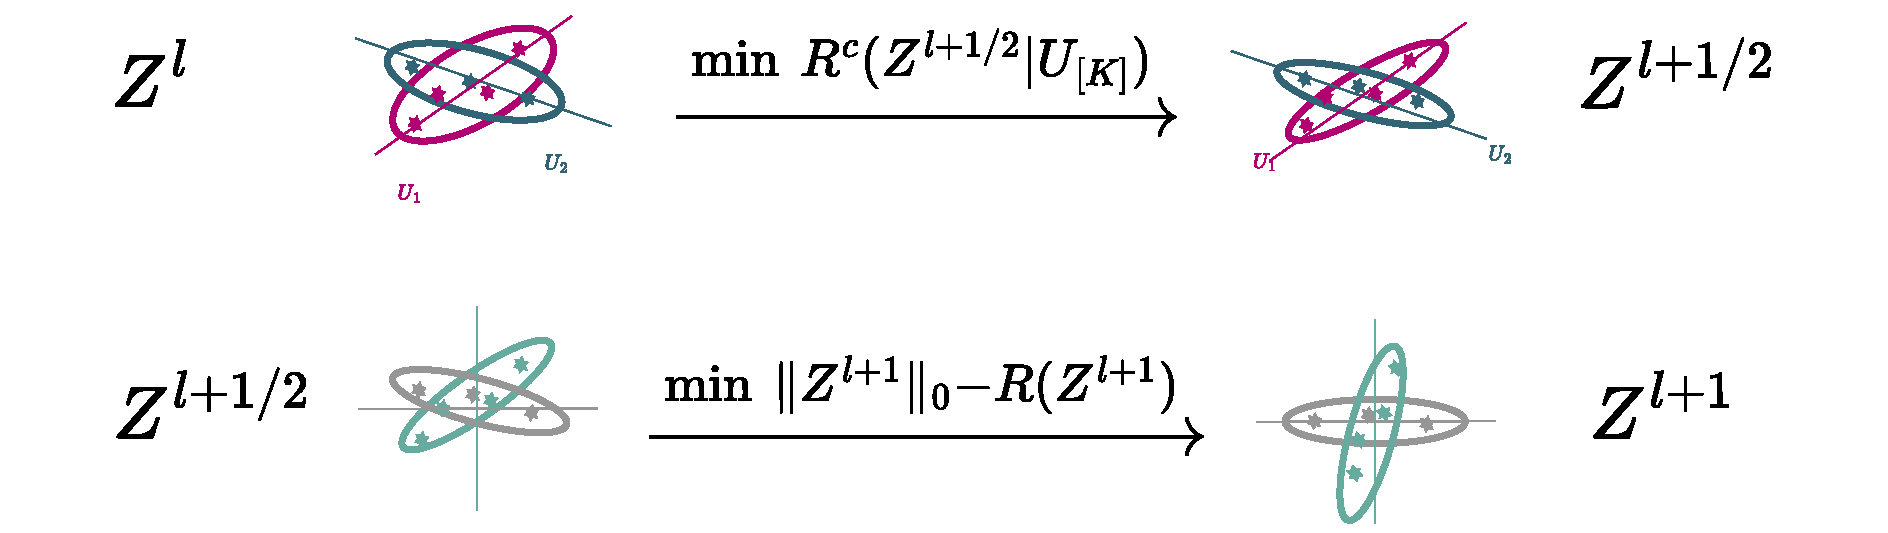
\includegraphics[width=0.75\textwidth]{imaxes/scrr.drawio.pdf}
	\caption{Iteración dos pasos do \acrshort{mcr2}}
  \label{fig:funcions_activacion}
\end{figure}

\subsection{ViT}
\section{Introdución a conceptos}
\subsection{Aprendizaxe de diccionarios}
\subsection{Aprendizaxe desenrolado}
\subsection{CRATE}
\label{subsec:crate}
\subsection{Conxuntos de datos}
\begin{figure}[htbp]
    \centering

    \begin{subfigure}{0.24\textwidth}
        \centering
        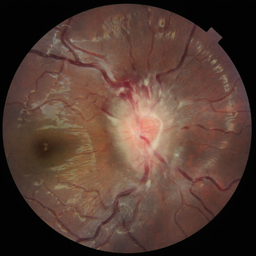
\includegraphics[width=\linewidth]{imaxes/rfmid.png}
        \caption{}
    \end{subfigure}
    \hfill
    \begin{subfigure}{0.24\textwidth}
        \centering
        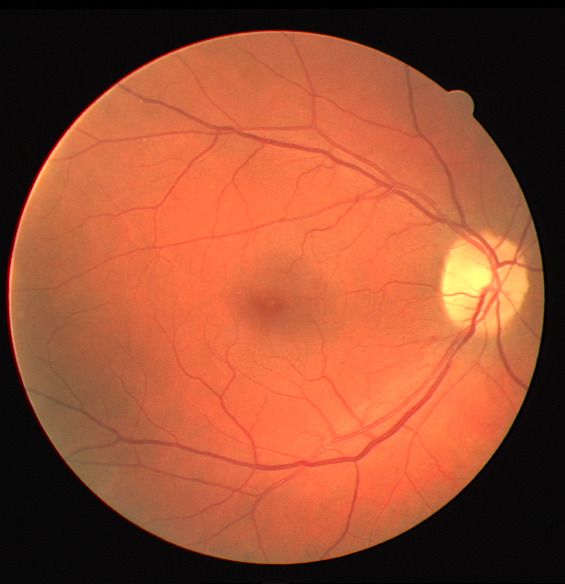
\includegraphics[width=\linewidth]{imaxes/drive_imaxe.jpg}
        \caption{}
    \end{subfigure}
    \hfill
    \begin{subfigure}{0.24\textwidth}
        \centering
        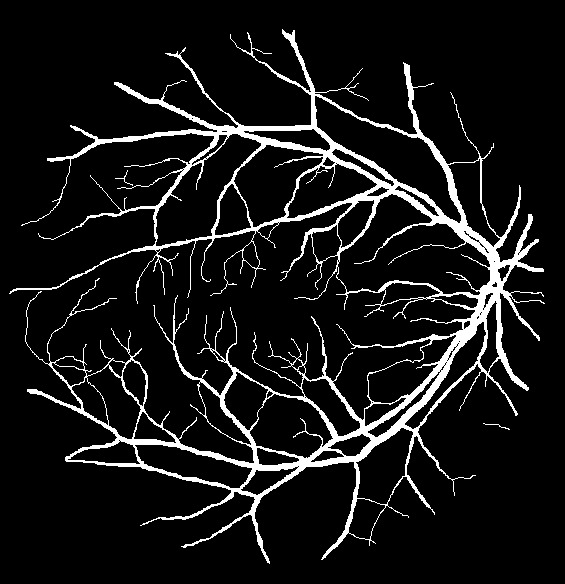
\includegraphics[width=\linewidth]{imaxes/drive_mascara.jpg}
        \caption{}
    \end{subfigure}
    \hfill
    \begin{subfigure}{0.24\textwidth}
        \centering
				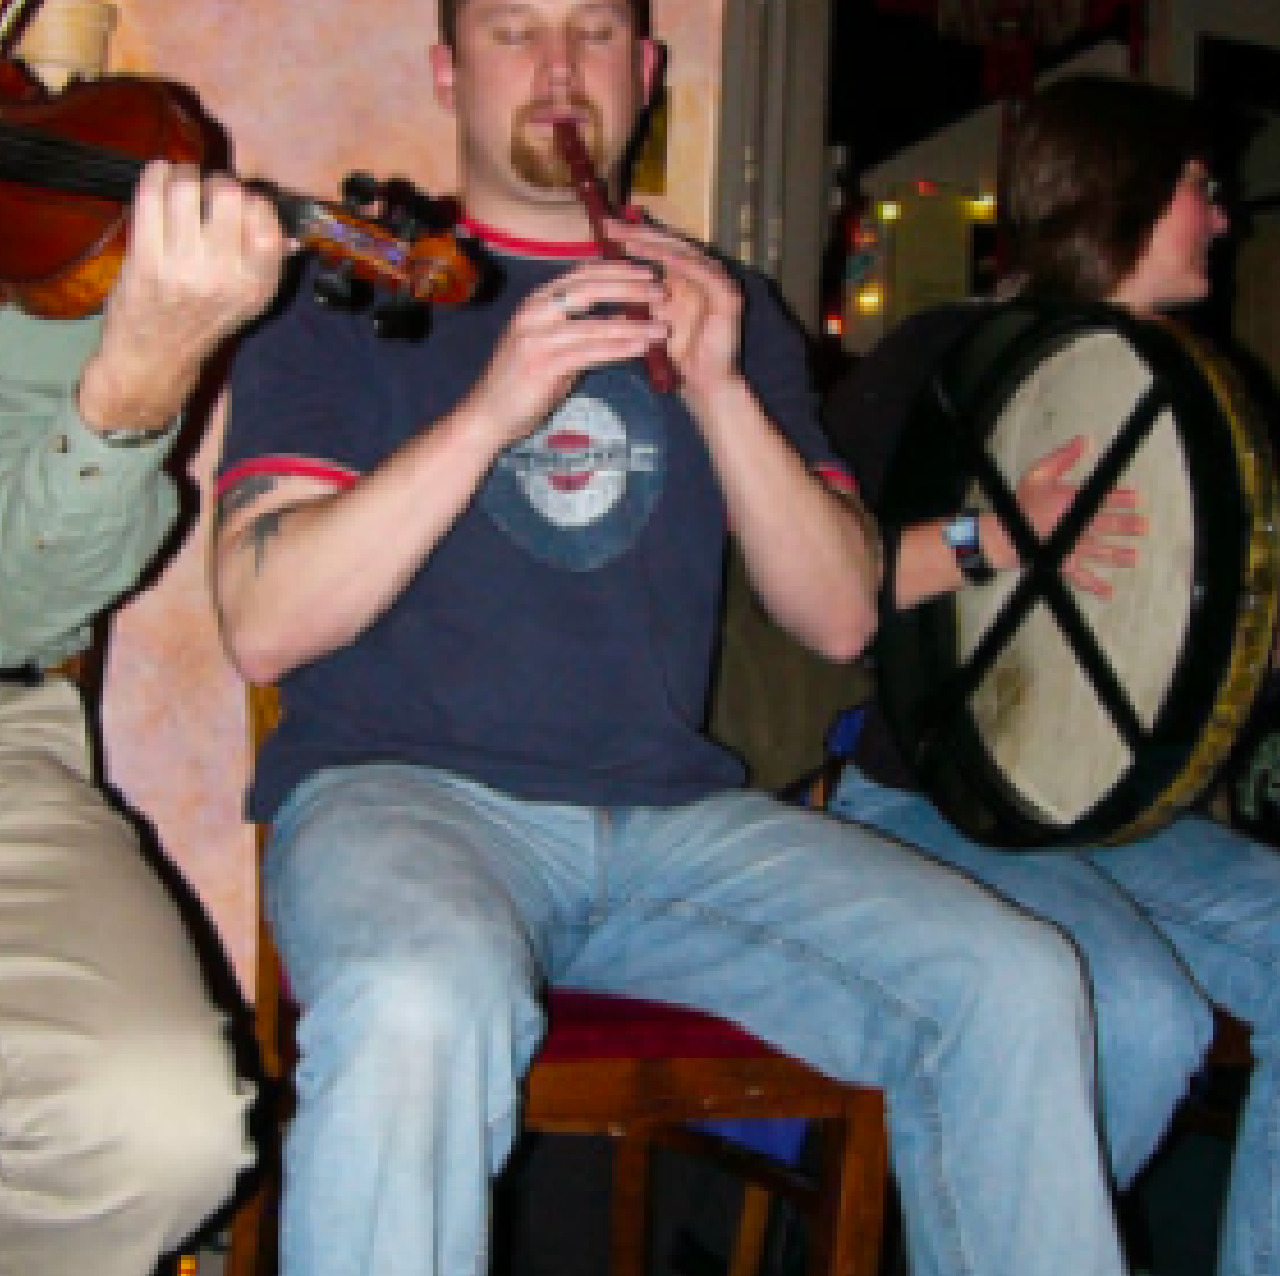
\includegraphics[width=\linewidth]{imaxes/imagenet.jpeg}
        \caption{}
    \end{subfigure}

    \caption{Mostras dos conxuntos de datos. (a) Imaxe de fondo de retina con edema de disco óptico, pertencente ó conxunto de datos RFMiD. (b-c) Imaxe de fondo de retina e a súa correspondente máscara binaria anotada, pertencentes ó conxunto de datos DRIVE (d) Imaxe de mostra do conxunto de datos ImageNet}
		\label{fig:datasets}
\end{figure}

\begin{itemize}
					\item \textbf{RFMiD 2.0 (2023).} \cite{rfmid} Recolle mostras de enfermidades raras con imaxes de alta resolución. Ademáis de a etiqueta `san', inclue 48 condicións entre as que se atopan as patoloxías vasculares (e.g. oclusións de veas e arterias, retinopatía hipertensiva, retinopatía hemorráxica, vasos tortuosos \dots), diabéticas (e.g. retinopatía diabética, edema macular, manchas algodonosas, microaneurismas \dots), dexenerativas ou relacionadas ca idade (e.g. dexeneración macular asociada ca idade, drusas, retinite pigmentaria, miopía \dots), trastornos do nervio óptico (e.g. escavación do nervio óptico, edema do disco óptico, palidez do disco óptico, hialose asteroide \dots), alteracións estructurais da retina (e.g. desprazamento da retina, burato retiniano, rotura retiniana \dots), congénitas (e.g. coloboma, pregamentos coroideos, hipertensión intracranial idiopática \dots) \dots Polo que é de gran utilidade para o diagnóstico e caracterización destas patoloxías dado o seu nivel de precisión cas etiquetas.
				\item \textbf{DRIVE (2004).} \cite{drive} Deseñado para segmentación de vasos sanguíneos, inclue 40 imaxes cas súas máscaras binarias anotadas manualmente por expertos (ver Figura \ref{fig:datasets} (b-c)).
					\item \textbf{ImageNet (2009).} \cite{imagenet} Nace ante a necesidade dun gran conxunto de datos de imaxe natural e foi plantexado como unha xerarquía de xeito que o concepto de \textit{clase} é multinivel, porque se ben hai animais e artefactos, ambos divídense en subcategorías recursivamente ate chegar ó nivel do individuo. É dicir, preséntase o `labrador alemán' non como un elemento illado pero como parte dos `cans' e estes á súa vez de `carnívoros', `placentarios'... Polo seu gran tamaño é variedade tivo un impacto notable no desenvolvemento do \acrshort{aprpro} es as \acrshort{rna}.
\end{itemize}

\section{Discusión}
\subsection{Elementos diferenciais}
\subsection{Oportunidades}
\subsection{Contribucións}
